% section
\section{Machine Learning Theory}
 % subsection
 \subsection{Image Prediction}
  \begin{frame}
   \frametitle{Image Prediction}
   
   \begin{itemize}
    \item<1-> Field inside machine learning / computer vision
    \item<2-> Predict future image/s, given sequence of images
    \item<3-> $X$ the image sequence of length $n$
    \item<4-> with $X = (x_0, \ldots, x_{n-1})$
    \item<5-> Two possible use-cases
    \begin{itemize}
     \item<6-> One-frame prediction
     \begin{itemize}
      \item<7-> Predicting $x_n$
     \end{itemize}
     \item<8-> Multi-frame prediction
     \begin{itemize}
      \item<9-> Predict $t > 1$ frames into the future $(x_n, \ldots, x_{n+t-1})$
      \item<10-> Often it is one-frame prediction in a feedback loop
      \item<11-> Propagate the error $\rightarrow$ Greater error in later images
     \end{itemize}
    \end{itemize}
   \end{itemize}
   
  \end{frame}
 
 % subsection
 \subsection{Autoencoder}
  \begin{frame}
   \frametitle{Autoencoder}
   
   \begin{itemize}
    \item<1-> Two networks chained together
    \begin{itemize}
     \item<2-> Encoder
      \begin{itemize}
       \item<3-> Input is $x$
       \item<4-> Output is $h$\footnote{$h$ is the so named \textbf{code}. Output layer is named \textbf{bottleneck layer}.}
       \item<5-> $E(x) = h$
      \end{itemize}
     \item<6-> Decoder
     \begin{itemize}
      \item<7-> Input is $h$
      \item<8-> Output is $x\prime$
      \item<9-> $D(h) = x\prime$
     \end{itemize}
    \end{itemize}
    \item<10-> Used for reconstruction $x \approx x\prime$
    \item<11-> Important is to prevent the network to simply copy $x$ to $x\prime$ (Interpolation)
    \item<12-> Simplest architecture is the undercomplete autoencoder
    \begin{itemize}
     \item<13-> Code smaller then input
     \item<14-> Network needs to distinguish between useful and obsolete
    \end{itemize}
   \end{itemize}
  
  \end{frame}
  \begin{frame}
   \frametitle{Autoencoder}
   
   \begin{figure}[H]
    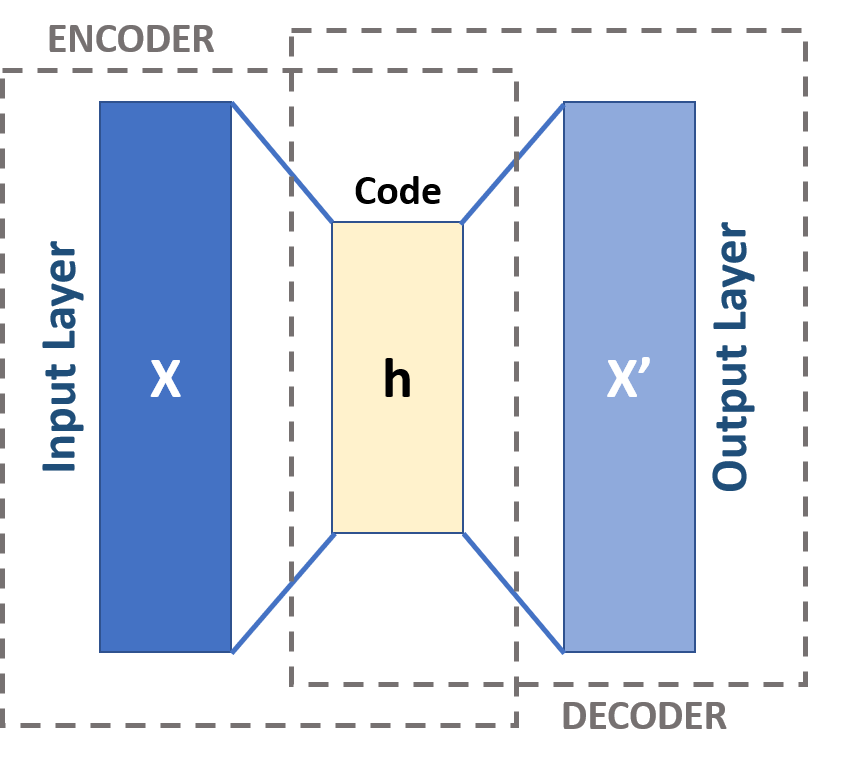
\includegraphics[width=0.38\textwidth]{../Images/autoencoder_schema.png}
    \centering
    \caption{Autoencoder schema \cite{wiki2019}}
    \label{fig:lstm_architecture}
   \end{figure}
   
  \end{frame}
 
 % subsection
 \subsection{CNN}
  \begin{frame}
   \frametitle{CNN}
   
   \begin{itemize}
    \item<1-> Convolutional Neural Network
    \item<2-> Consists of three stages
    \begin{enumerate}
     \item<3-> Convolutional layer
     \item<4-> Non-linearity (ReLU, sigmoid, $\ldots$)
     \item<5-> Pooling layer
    \end{enumerate}
   \end{itemize}

  \end{frame}
  \begin{frame}
   \frametitle{CNN (First stage)}
   
   \begin{itemize}
    \item<1-> Convolutional operation is discrete
    \item<2-> $(I \ast K)(i,j) = \sum_m\sum_nI(m,n)K(i-m,j-n)$
   \end{itemize}
   \onslide<3->{
   \begin{figure}[H]
    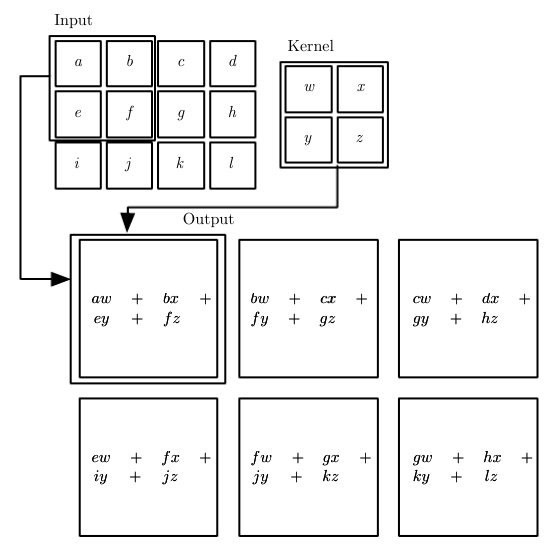
\includegraphics[width=0.45\textwidth]{../Images/kernel.png}
    \centering
    \caption{Two dimensional convolutional operation \cite{Goodfellow2016}}
    \label{fig:kernel}
   \end{figure}
   }
   
  \end{frame}
  \begin{frame}
   \frametitle{CNN (Second stage)}
   
   \begin{itemize}
    \item<1-> 
   \end{itemize}
   
  \end{frame}
 
 % subsection
 \subsection{RNN}
  \begin{frame}
   \frametitle{RNN}
   
  \end{frame}
 
 % subsection
 \subsection{LSTM}
  \begin{frame}
   \frametitle{LSTM}
   
  \end{frame}
 
 % subsection
 \subsection{ConvLSTM}
  \begin{frame}
   \frametitle{ConvLSTM}
   
  \end{frame}
 
 % subsection
 \subsection{Backpropagation}
  \begin{frame}
   \frametitle{Backpropagation}
   
  \end{frame}

 % subsection
 \subsection{BPTT}
  \begin{frame}
   \frametitle{BPTT}
   
  \end{frame}  
